\documentclass{article}
\usepackage{amsmath}    % loads AMS-Math package
\usepackage{graphicx}   % allows image files
\usepackage{listings}   % allows lstlisting environment
\usepackage[letterpaper, margin=0.75in]{geometry}  % set paper size/margins
\usepackage{EGR103style}% colorful file imports
\usepackage{tikz}
\usepackage{multicol}
\usepackage{xcolor}
\usepackage{parskip}
\usepackage{caption}
\usepackage{wrapfig}

% Colors
\definecolor{dukeBlue}{HTML}{0033A0}
\definecolor{ncRed}{HTML}{C8102E}
\definecolor{panelGray}{HTML}{F6F7F9}
\definecolor{accentBlue}{HTML}{5B8FF9}
\definecolor{accentRed}{HTML}{FF6B6B}


\begin{document}
\begin{center}
\rule{6.5in}{0.5mm}\\~\\
\textbf{\large Duke University}\\[.75em]
\textbf{\large ME421 -- Fall 2025}\\[1em]
\textbf{\huge State Fair Project} \\[.75em]
\textit{\LARGE Ball Durham}\\[1.5em]

Emilie Steinberg (es468), Gretchen Houser, Trey Fitzpatrick (mjf74), Ryan Christ (rjc70), Dylan Matian (drm71) \\
\rule{6.5in}{0.5mm}\\
\end{center}
\tableofcontents

\section{Small Scale Poster}

\begin{figure}[h]
\begin{center}
     \includegraphics[width=1\textwidth]{info2.png}
\end{center}
\end{figure}
\clearpage
\section{Final BOM, Overall and Filament}
\begin{figure}[h!]
\begin{center}
     \includegraphics[width=1\textwidth]{FinalBOM.png}
\end{center}
\end{figure}
\begin{figure}[h!]
\begin{center}
     \includegraphics[width=0.8\textwidth]{FilamentCost.png}
\end{center}
\end{figure}
\clearpage

\section{Project Budget BOM}
\begin{figure}[h!]
\begin{center}
     \includegraphics[width=1\textwidth]{bom1.png}
\end{center}
\end{figure}
\section{Final Testing Results}
After fully assembling our pinball machine, our team went through various testing to ensure rigidity of our mechanisms and make sure it is intuitive to play. Part of testing focused on durability by repetitively playing with it to simulate use by children at the state fair, as well as usability improvements based on our performance. We first tested it by repetitively playing with it to verify that all mechanisms could withstand the forces from continuous use without breaking. One of our findings was that the launch mechanism created significant forces on the machine when users pulled back the spring plunger. To address this, we added triangular support braces cut at 45 degrees at the front and back of the machine. These braces improved stability and prevented the structure from rocking and shifting when pulling back the launcher. Additionally, during our testing, we noticed that the balls could occasionally escape from the bottom sides of the machine. To resolve this issue, we installed wooden guide pieces along the bottom besides ball catcher area to prevent ball from falling below, while also funneling the balls toward the retrieval area. Finally, we noticed that it was very hard to get the ball inside the hoop with our initial ramp design. To resolve this, we modified the ramp by increasing both its width and length, making it easier for players to get the ball in the hoop. By the end of testing, all of our mechanisms showed reliable performance making it ready for the public.

\section{Appendix}
\subsection{Component and Material Summary}
\subsubsection{Wooden Exterior/Board}
For the exterior of our machine, we wanted a material that was lightweight and easy to cut. After considering several options, we chose Plywood because it is cost-effective and can be found on campus. To construct the outer frame, we will use about two pieces measuring {3}{ft} $\times$ {2}{ft} $\times$ {0.25}{in}, one piece measuring {5}{ft} $\times$ {2}{ft} $\times$ {0.25}{in}, and one piece measuring {5}{ft} $\times$ {3}{ft} $\times$ {0.25}{in}. For the main playfield, we require a solid block of plywood measuring {3}{ft} $\times$ {5}{ft} $\times$ {6}{in}, which will provide the necessary slope and structural support.
\\
\\
The board is set at a $7^\circ$ angle (as shown in \textit{Section 6.1.1, Hand Calculations}) and is fastened to the wooden exterior. This creates a hollow area under the board, allowing room for integration of the ramp component and other launch mechanisms. The ramp then guides the ball back to the front of the machine, allowing players to reset quickly for the next round. 
\subsubsection{Board Pins and Final Integration Layout}
The pins are designed to direct the ball toward the flippers and guide it back to the hoop. The pins also reflect the basketball theme, featuring Duke and NC State designs. For fabrication, we plan to 3D print each pin using standard PLA material. Detailed dimensions for the pins can be found in the 'Part Drawings' Appendix.
\vspace{1em}
\\
* \textit{See the image below to see the final board design:}

\begin{figure}[h]
\begin{center}
     \includegraphics[width=.9\textwidth]{final.png}
\end{center}
\end{figure}
\clearpage
\subsubsection{Launch Mechanism}
\begin{figure}[h]
\begin{center}
     \includegraphics[width=.7\textwidth]{launchmechanism2.png}
\end{center}
\end{figure}

The launch mechanism is designed to provide players with a consistent, controllable way to introduce the ball into play. To achieve this, we implemented a spring-powered system, similar to those used in traditional pinball machines. The system consists of a cylindrical guide channel, a compression spring, and a conical handle, damping foam, and force bearing attachment. The spring stores potential energy when compressed by the user and converts it into kinetic energy to accelerate the ball along the launch lane once released. The head, tip, and rod are all fixed using set screws to an aluminum rod with flattened portions the set screw is preloaded to. The only force bearing component here is the spring. 

\begin{table}[htbp]
\centering
\renewcommand{\arraystretch}{1.3}
\begin{tabular}{|c|c|}
\hline
\textbf{Parameter} & \textbf{Value} \\ \hline
Spring Inner Diameter (ID) & 0.51 in \\ \hline
Spring Outer Diameter (OD) & 0.60 in \\ \hline
Spring Free Length & 3.50 in \\ \hline
Compressed Spring Length @ Max Load & 1.269 in \\ \hline
Spring Constant ($k$) & 2.7 lb/in \\ \hline
Ball Mass ($m$) & 0.17637 lb \\ \hline
\end{tabular}
\caption{Spring specifications and ball mass. Data from McMaster-Carr.}
\end{table}

\begin{equation}
F_{spring,\space  max} = kx_{spring. \space max}
\end{equation}

\begin{equation}
x{_spring, \space max} = L_{\text{free}} - L_{\text{compressed}} = 3.50 - 1.269 = 2.231 \ \text{in}
\end{equation}

\begin{equation}
F = (2.7 \ \text{lb/in})(2.231 \ \text{in}) = 6.02 \ \text{lb}
\end{equation}

Next, applying conservation of energy we can find ball speed at max compression

\begin{equation}
\frac{1}{2}kx^2 = \frac{1}{2}mv^2
\end{equation}

\begin{equation}
v = \sqrt{\frac{kx^2}{m}} = \sqrt{\frac{(2.7 \ \text{lb/in})(2.231 \ \text{in})^2}{0.17637  \ \text{lb}}} = 8.729 \ \text{in/s}
\end{equation}

\newpage
\subsubsection{Ramp Return Mechanism}
In order to get the ball back to the player, we needed to design a ramp. This addition allows players to reuse their ball if they make it in the basket or miss the flippers. The height of the ramp was made to match the 7 degree angle of the board. This was done to ensure that when the ball drops, it can will fall in the same line as it does when missing the flippers. 
\vspace{1em}
\\
* \textit{See the image below to see a transparent view of the ramp system under the board:}

\begin{figure}[h]
\begin{center}
     \includegraphics[width=1.0\textwidth]{ramptrans.png}
\end{center}
\end{figure}
\newpage
\subsubsection{Hoop Flag Mechanism}
The hoop is designed as a target for the players to hit the ball into, and upon the ball falling into the hoop, it will hit a lever that will trigger a mechanism using two torsional springs to release a flag, indicating victory. The hoop and block-looking parts will be 3D printed, and the flag rod and reset mechanism will be made with wooden dowels. In order to avoid complex assumptions and calculations, the lever will be weighted such that the mechanism triggers properly. The CAD for the mechanism is shown below: 

\begin{figure}[h]
\begin{center}
     \includegraphics[width=1.0\textwidth]{HoopMechanism.png}
\end{center}
\end{figure}

Unfortunately during final integration there was not enough time to integrate all of the mechanisms, so the decision was made to remove the flag functionality and simply install the hoop and mount components without the added mechanical complications of the flag pop-up system. While the initial idea was to weight the pendulum so as to make the ball falling trigger the mechanism, after beginning to build the mechanism it was found that it would be more effecient to weight the down position lever-arm in order to create the proper set-point. The platform with the mechanisms in their final iteration, pre-integration are shown below:
\begin{figure}[h] 
    \centering
    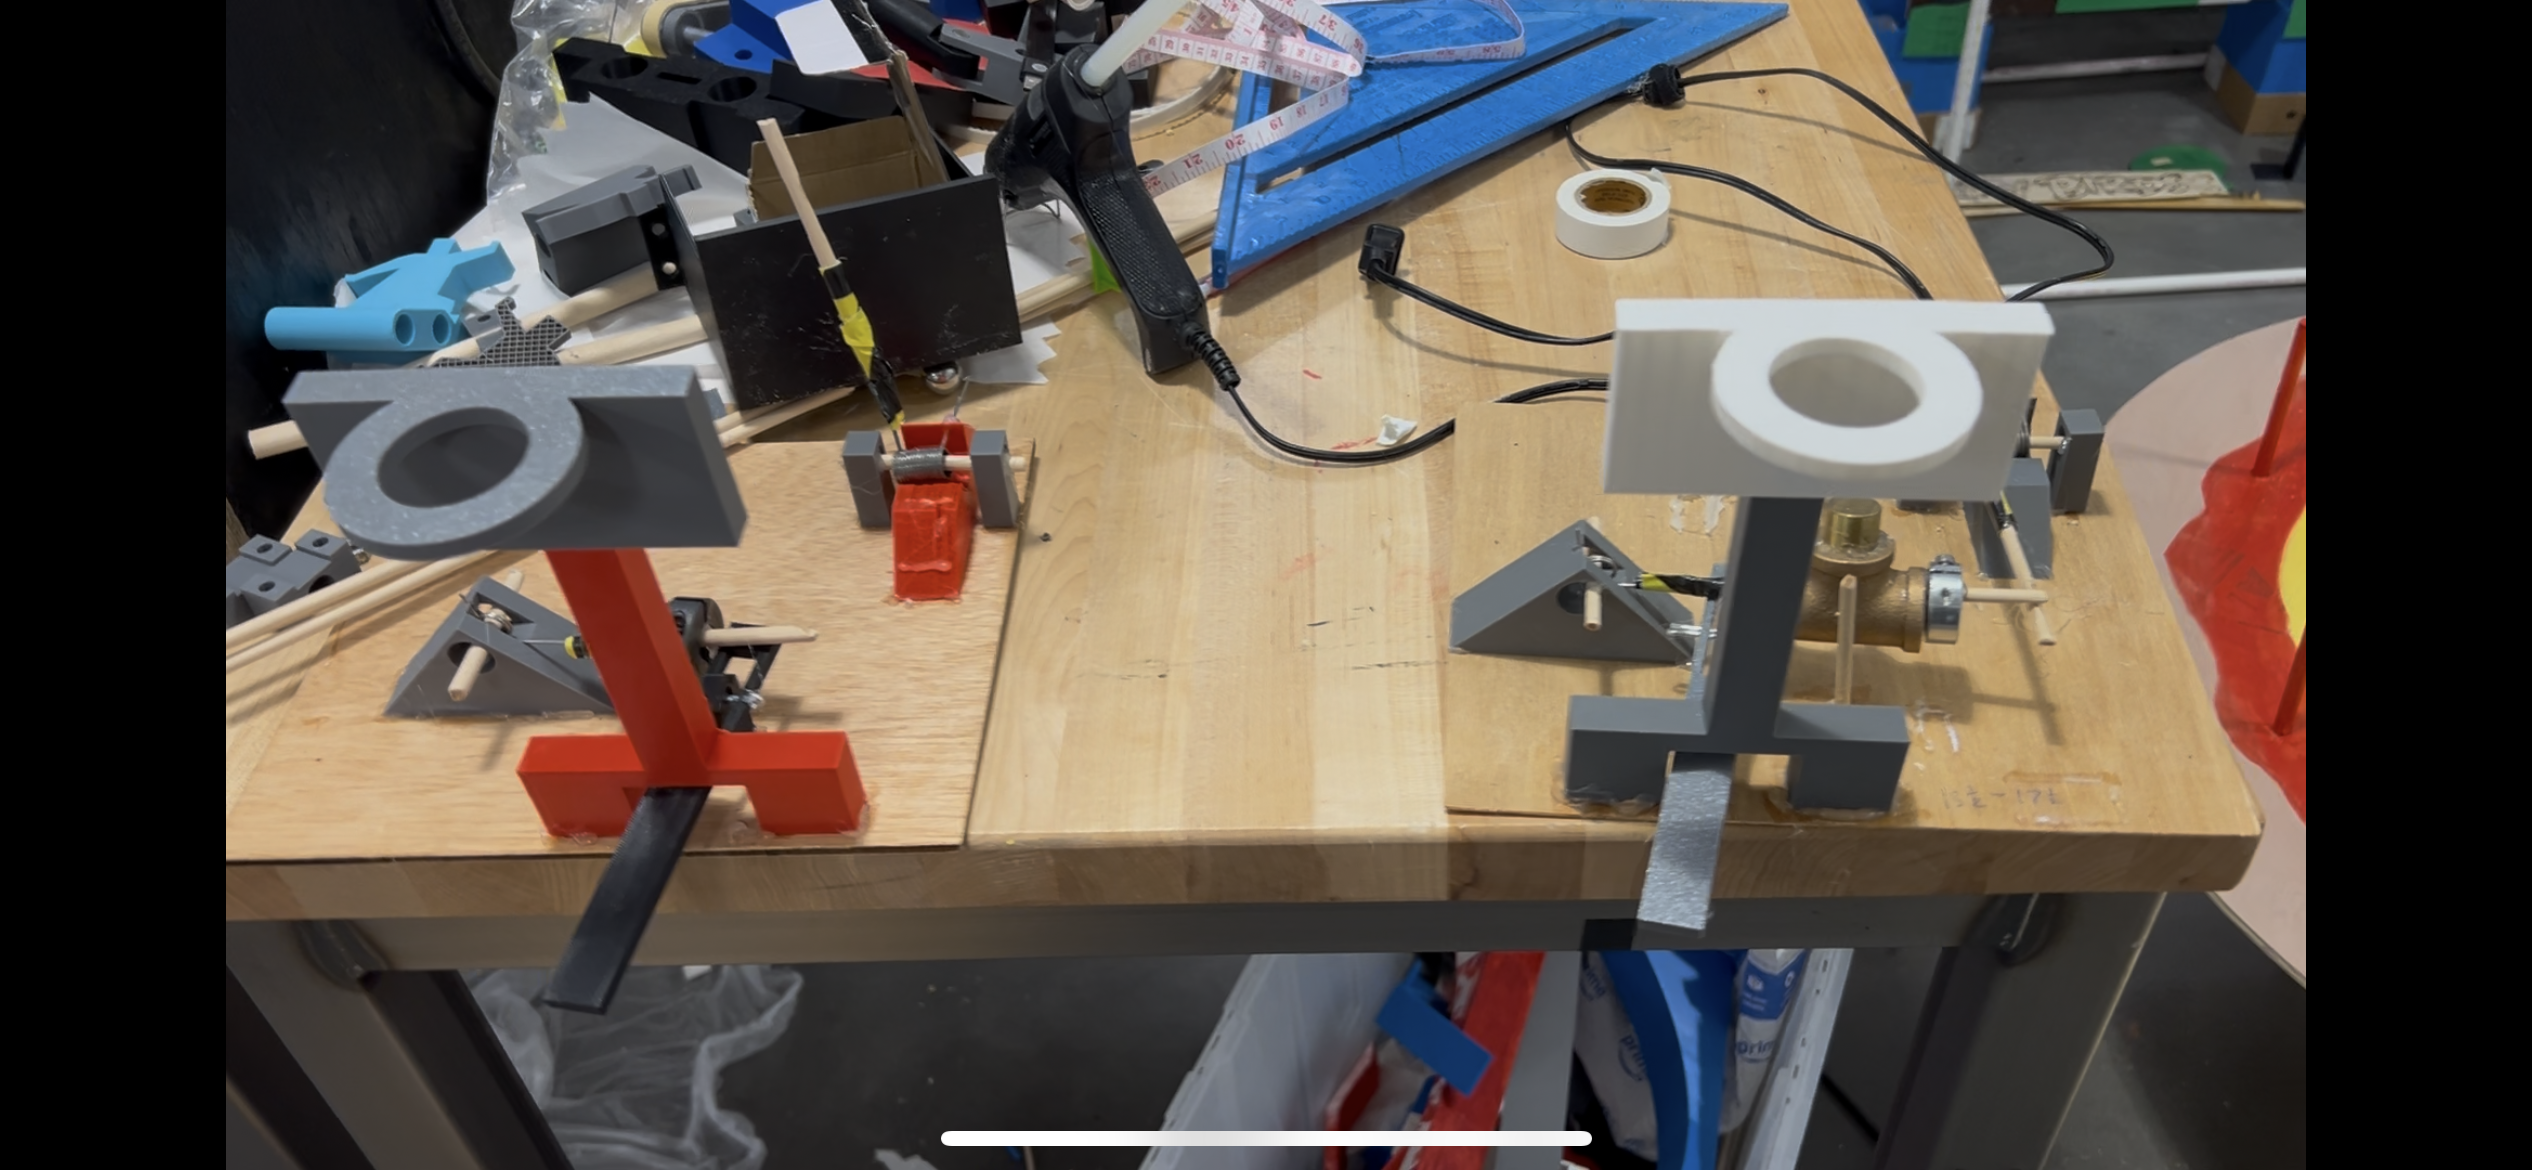
\includegraphics[width=1\textwidth]{AsBuiltFlag.PNG}
    \caption{Flag Mechanisms}
\end{figure}
\newpage
\subsubsection{Flipper and Handle Mechanism}

The flipper is mounted to a central steel rod that acts as the rotational axis (aligned with the $\vec{u_2}$-axis). This rod passes through the pinball board and is supported by a press-fit ball bearing. The flipper will be 3D printed and wrapped with a thin rubber sleeve so that the ball makes consistent contact with the paddle. Under of the board, the same rod connects to a 3D-printed lever arm of length $d_h = 1.3545$\,in. The free end of the lever is connected to the user’s handle by a steel dowel pin, which allows slight movements as the handle slides while still constraining the lever to rotate with the rod. The handle is also 3D printed. As the user pushes or pulls the handle, the dowel pin forces the lever to rotate, and therefore the flipper rotates by the same angle. A return spring is attached beneath the board, where one end is fixed to the wooden frame, the other to the lever at a distance, $d_s = 1.397$\,in from the shaft. This spring provides a restoring torque that returns the flipper to its rest position when released.

\noindent The relationship between the linear travel $s$ of the handle and the angular rotation $\theta$ of the flipper is:
\[s(\theta) = d_h \sin\theta, \qquad \theta(s) = \arcsin\!\left(\tfrac{s}{d_h}\right).\]
\noindent The governing equation of motion for the flipper shaft is:
\[I \ddot{\theta}(t) = -k d_s^2 \,\theta(t) + F_{\text{user}}\, d_h,\]
\noindent See image below for the CAD model and the Appendix for the FBD of the mechanism.

\begin{figure}[ht]
\begin{center}
     \includegraphics[width=0.75\textwidth]{CAD_Flipper.png}
     \caption{CAD Design of the Flipper Mechanism}
\end{center}
\end{figure}

\
\subsubsection{Defender Mechanism}
In order to add a competitive and interactive aspect to the game, a defender mechanism was designed for both sides. The mechanism consists of two mirrored bodies with flaps (positioned 135$^{\circ}$ from the bodies), two wooden dowels (one of which is fixed to the board via 3D printed pins), a button, a PVC lever, and a bracket that guides the lever along the plane of the board. The mechanism was integrated using the jigsaw to cut out the shape of the bodies from the board surface. See below for assembly and appendix for engineering drawings. 
\begin{figure}
    \centering
    \includegraphics[width=0.75\textwidth]{Defender side view.png}
    \caption{CAD assembled defender mechanism for Duke side}
    \label{fig:placeholder}
\end{figure}
\begin{figure}
    \centering
    \includegraphics[width=0.75\textwidth]{Defender top view.png}
    \caption{CAD assembled defender mechanism top view}
    \label{fig:placeholder}
\end{figure}
To combat board clearance issues, the final defender design was thinned to .45" in thickness. This design required less material to be cut from the board, allowing the ball to roll more smoothly over the defenders when not activated. Additionally, because the defenders are controlled by the opposite side's player, a PVC elbow was added to one lever to avoid contact with the mechanisms. These elbows were adhered using PVC cement and primer. Pictured below is the final  elbow/lever assembly visible under the board. 
\\
\\
\noindent When the button is pushed, the defenders rotate until they are stopped (by the cut in the board) in an upright position. While iterating, a .015" tolerance was added to the holes in the defenders, which allowed the wooden dowels to rotate relatively freely. Additionally, in the final assembly, washers were added to constrain the defenders from horizontal motion. The longer wooden dowel was super glued to the PVC lever so that the assembly will move as one unit. Due to the weight of the defender bodies, when the button is released, they fall back into "off" position, or flush with the board's surface. 
\\
The pin brackets are attached with 1/4"-20 wood screws with 1 1/2" length. Because these screws were obtained from Duke's supply, and no shorter length was available, the brackets were designed with added thickness to prevent the screws from protruding into the board's surface. A comparable wood screw is Mcmaster Carr part 91087A124, priced at \$.41 per screw. The lever brackets are attached with 3/8" diameter, 1 1/2" length wood screws. A similar part from Mcmaster Carr is part 92351A628, priced at \$.76 per screw.
\begin{figure}
    \centering
    \includegraphics[width=0.75\textwidth]{under board.jpeg}
    \caption{Assembly under board surface}
    \label{fig:placeholder}
\end{figure}


\clearpage
\subsection{First Stage Build}
\begin{figure}[h] 
    \centering
    \includegraphics[width=.5\textwidth]{first.png}
\end{figure}

\subsection{Final Machine}
\begin{figure}[h] 
    \centering
    \includegraphics[width=.5\textwidth]{mac.png}
   
\end{figure}
\clearpage
\subsection{Calculation Summary}
\subsubsection{Hand Calculations}
\begin{figure}[h] 
    \centering
    \includegraphics[width=.9\textwidth]{BoardCalcs.png}
    \caption{Sizing Board and Exterior Structure Calculations}
\end{figure}
\clearpage
\begin{figure}[ht]
\begin{center}
     \includegraphics[width=0.75\textwidth]{Flipper_Mechanism.jpg}
     \caption{Flipper Mechanism FBD and EQM Derivation}
\end{center}
\end{figure}
\clearpage
\subsubsection{Piece Part Drawings}
\begin{figure}[h] 
    \centering
    \includegraphics[width=1\textwidth]{Back.png}
    \caption{Backboard drawing}
\end{figure}
\begin{figure}[h] 
    \centering
    \includegraphics[width=1\textwidth]{front.png}
    \caption{Front board drawing}
\end{figure}
\begin{figure}[h] 
    \centering
    \includegraphics[width=1\textwidth]{front.png}
    \caption{Exit hole drawing}
\end{figure}
\clearpage
\subsubsection{Ramp}
\begin{figure}[h] 
    \centering
    \includegraphics[width=1\textwidth]{ramp.png}
    \caption{Ramp Return drawing}
\end{figure}
\clearpage
\subsubsection{Board Pins}

\begin{figure}[h] 
    \centering
    \includegraphics[width=1\textwidth]{launcher.png}
    \caption{Launcher pin drawing}
\end{figure}
\begin{figure}[h] 
    \centering
    \includegraphics[width=1\textwidth]{left launch.png}
    \caption{Left flipper guide drawing}
\end{figure}


\begin{figure}[h] 
    \centering
    \includegraphics[width=1\textwidth]{right launch.png}
    \caption{Right flipper guide drawing}
\end{figure}
\begin{figure}[h] 
    \centering
    \includegraphics[width=1\textwidth]{Nc.png}
    \caption{NC Logo Pin drawing}
\end{figure}
\begin{figure}[h] 
    \centering
    \includegraphics[width=1\textwidth]{TopofBoard.png}
    \caption{Top of Board Drawing drawing}
\end{figure}
\begin{figure}[h] 
    \centering
    \includegraphics[width=1\textwidth]{Top Obstacle.png}
    \caption{Top Obstacle Pin drawing}
\end{figure}
\subsubsection{Hoop Components}
\begin{figure}[h] 
    \centering
    \includegraphics[width=1\textwidth]{HoopMountDrawingFinal.JPG}
    \caption{Hoop Mount drawing}
\end{figure}
\begin{figure}[h] 
    \centering
    \includegraphics[width=1\textwidth]{HoopPartFinal.JPG}
    \caption{Hoop Part drawing}
\end{figure}

\clearpage

\subsubsection{Assembly Drawings + Transparent Views}
\begin{figure}[h] 
    \centering
    \includegraphics[width=1\textwidth]{HoopDrawing.jpg}
    \caption{Hoop Mechanism Drawing}
\end{figure}
\begin{figure}[h] 
    \centering
    \includegraphics[width=1\textwidth]{Pinball_Flipper_Assembly_Left- Drawing 1.png}
    \caption{Flipper Mechanism Drawing}
\end{figure}
\begin{figure}[h] 
    \centering
    \includegraphics[width=1\textwidth]{assenbly 2.png}
    \caption{Assembly drawing}
\end{figure}
\begin{figure}[h] 
    \centering
    \includegraphics[width=1\textwidth]{DEFENDER.png}
    \caption{Defender drawing}
\end{figure}
\begin{figure}[h] 
    \centering
    \includegraphics[width=1\textwidth]{button 2.png}
    \caption{Button drawing}
\end{figure}
\begin{figure}[h] 
    \centering
    \includegraphics[width=1\textwidth]{pin bracket 3.png}
    \caption{Pin bracket drawing}
\end{figure}

\begin{figure}[h] 
    \centering
    \includegraphics[width=1\textwidth]{lever bracket 3.png}
    \caption{Lever bracket drawing}
\end{figure}

\begin{figure}[h] 
    \centering
    \includegraphics[width=1\textwidth]{launchmechanismDrawing.pdf}
    \caption{Launch Mechanism}
\end{figure}

\begin{figure}[h] 
    \centering
    \includegraphics[width=1\textwidth]{BomAssy.png}
    \caption{BOM + Assembly Drawing}
\end{figure}

\end{document}